
\documentclass[12pt,a4paper,titlepage]{article}
\usepackage{amsmath}
\usepackage{latexsym}
\usepackage{amssymb}
\usepackage{amstext}
\usepackage{nccmath}
\usepackage{mathtools}
\usepackage{array}
\usepackage{fixmath}
\usepackage{mathrsfs}
\usepackage{pdfpages}

\setlength{\textwidth}{15cm} \setcounter{page}{159}

\begin{document}


\begin{titlepage}
    \begin{center}
        \vspace*{3.5cm}
        
        \textbf{\huge{Forschungspraxis Proposal}}
        
        \vspace{8cm}

        \begin{verse}
            \ \ \ \ \ \ \ \ \ \ \ \ \ \ \ \ \ \ \ \ \ \ \ \ \ \textbf{\large{Student: Zhiwei Han}}\\
            \ \ \ \ \ \ \ \ \ \ \ \ \ \ \ \ \ \ \ \ \ \ \ \ \ \textbf{\large{Supervisor1: Hao Shen}}\\
            \ \ \ \ \ \ \ \ \ \ \ \ \ \ \ \ \ \ \ \ \ \ \ \ \ \textbf{\large{Supervisor2: Dominik Meyer}}\\
        \end{verse}


        
        \vspace{1cm}
        
%        \includegraphics[width=0.4\textwidth]{university} 
        
        Lehrstuhl f\"ur Datenverarbeitung\\
        Technische Universt\"at M\"unchen\\
        \today
        
    \end{center}
\end{titlepage}



\setlength{\parindent}{0pt} \setlength{\parskip}{2ex plus 0.5ex
minus 0.2ex}


\section*{1. Title}
\subsection*{1.1 Topic Description}
In this practical research, a well-designed efficient online TD learning algorithm will be introduced. This algorithm benefits from the sparsity, generated by $\ell1$ regularization, and high representation ability, provided by kernel method and aim at a more accurate and efficient value function approximation in machine learning problems.
\subsection*{1.2 Rough Title}
An Online Feature Select Kernel-Based TD Learning with $\ell1$ Regularization
\section*{2. Motivation}
The purpose of this practical research is trying to solve two main problems in reinforcement learning:\\

1. The performance of reinforcement learning algorithms relies heavily on the feature selecting of value function approximation. Even the most experienced experts can struggle with this task, therefore a proper representation approach is required . 

2. In traditional reinforcement learning algorithm, dimension explosion is still a limitation in large scale application like GO, because the computational complexity grows exponentially. The sparsity is one of proper solutions for the challenge of high computational expanse and memory consumption.
\newpage
\section*{3. Goal, Methodology and Verification}
The goal of this practical research is to find a more efficient way to solve both problems and to develop a new online TD learning algorithm, which is more efficient than the traditional TD algorithm with linear value function approximation from the perspectives of running time and memory consumption.\\

Although feature selection is usually limited by the understanding to problems, an appropriate expression of state can still be derived by using some specific kernel functions. The reason is kernel method can enrich trivial features by transferring the given features into high dimensional space and so that the kernel-based features will own more complex and accurate representation of states.\\

In the other hand, currently many studies are concentrating on reducing the computational expanse of large scale or complex problems and one well-known away is to use the sparsity generated by $\ell1$ regularization, which means, the coefficients of some correlated features will be replaced by 0. With that, the performance of learning algorithm will be greatly improved because much dirty computational work is reduced.\\

The efficiency of designed algorithm will be tested and verified through comparative experiment with standard TD algorithm with linear value function approximation on the problems mountain car and inverted pendulum. All the experiment will be done firstly on mathematical simulator and after verification it will be transmitted to reinforcement learning platform OpenAI Gym for visualization.

\newpage
\section*{4. Project Organization}
\subsection*{4.1 Schedule}
1. \textbf{Preparation}\\
a) Read the papers and learn the framework of kernel method and $\ell1$ regularization.\\
b) Set up the development environment include python and OpenAI Gym.\\

2. \textbf{Previous Work}\\
a) Analyze the problem and find the proper mathematical representation of them.\\
b) Finish the simulator algorithm.\\
c) Define state space.\\
d) Find several useful kernel functions.\\

3. \textbf{Algorithm Research}\\
a) Understand the framework of kernel function and $\ell1$ regularization used in reinforcement learning.\\
b) Develop and implement the main algorithm of this work and debug.\\
c) Try different kernel functions and choose one proper out of them.\\
d) Develop and implement the comparison algorithm and debug.\\
e) Intermediate report the result to supervisor.\\

4. \textbf{Efficiency Verification And Modification}\\
a) Test the functionality of two algorithms on simulator several times.\\
b) Compare the efficiency and debug.\\

5. \textbf{Visualization And Report Writing}\\
a) Transmit the functional algorithms onto reinforcement learning platform OpenAI Gym to simulate the real world condition for visualization.\\
b) Collect the learning information and note down the data.\\
c) Write the report and summarize the practical research.\\
\subsection*{4.2 Milestones}
1. State space definition design finished\\

2. Algorithm design finished\\

3. Proper kernel function found\\

4. Practical part ended
\subsection*{4.3 Time Table}
Please see attachment.
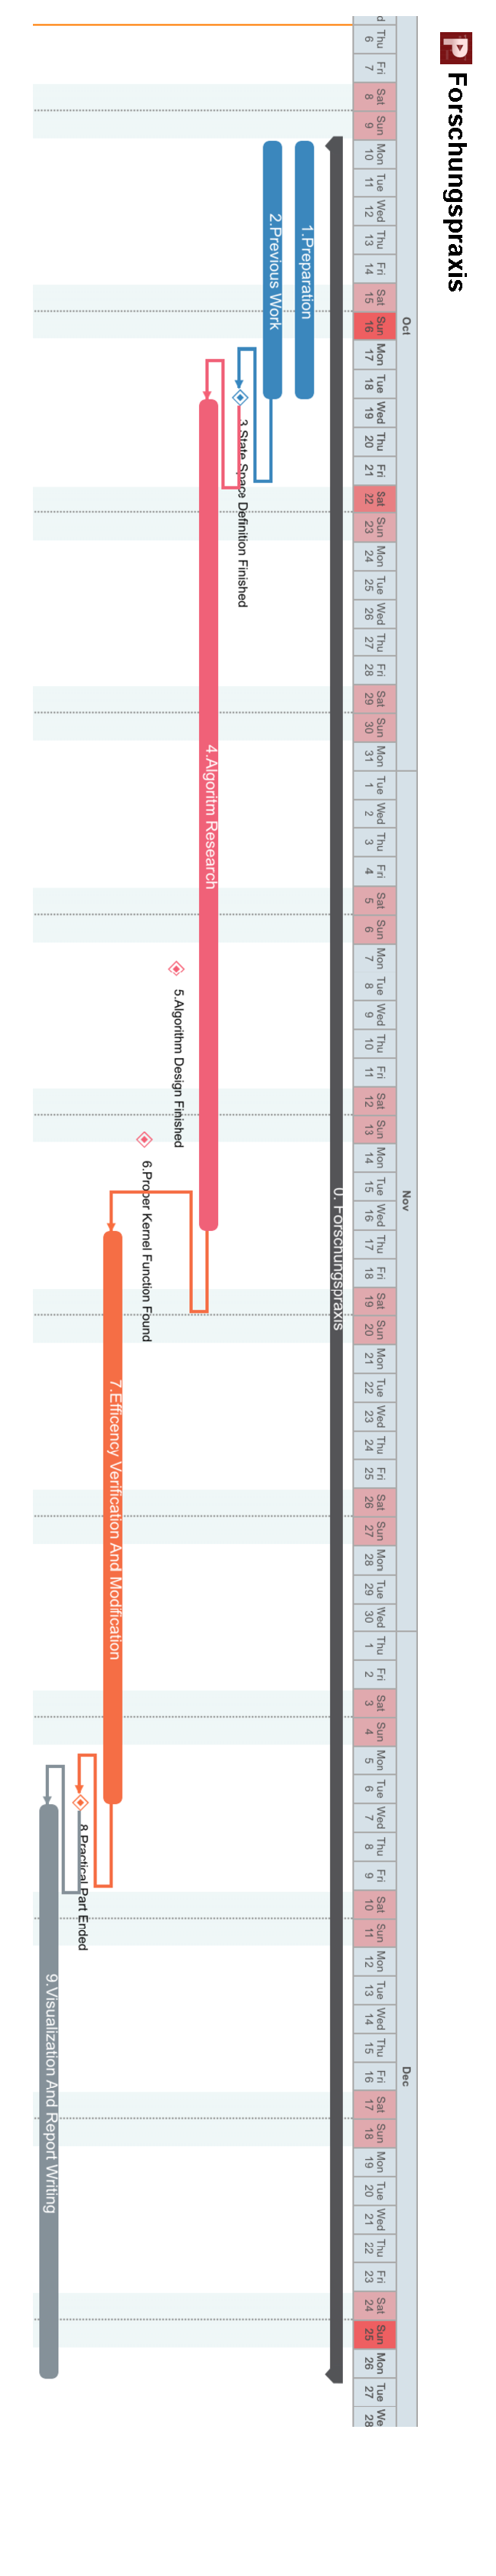
\includepdf[pages=-]{Schedule.pdf}
\end{document}
